\documentclass{beamer}
\usepackage{tikz}
\usetheme{Madrid}
\usepackage{ctex}
\usecolortheme{default}
\usepackage{verbatim}
\title[2022.11.21日汇报] %optional
{2022.12.5汇报}
%\subtitle{Demonstrating the Berkeley theme}
\author[周添文] % (optional)
{周添文\inst{} }

\institute[] % (optional)
{
  \inst{}%
  数学科学学院\\
  北京师范大学\\
 % \and
  %\inst{2}%
%  Faculty of Chemistry\\
%  Very Famous University
}

\date[2022.12.5] % (optional)
%{Very Large Conference, April 2021}

% Use a simple TikZ graphic to show where the logo is positioned

%\node[draw,color=white] at (0,0) {LOGO HERE};


%End of title page configuration block
%------------------------------------------------------------
%The next block of commands puts the table of contents at the 
%beginning of each section and highlights the current section:

\AtBeginSection[]
{
  \begin{frame}
    \frametitle{Table of Contents}
    \tableofcontents[currentsection]
  \end{frame}
}
%------------------------------------------------------------
\begin{document}
\frame{\titlepage}
%\logo{\includegraphics[]{bnu.png}}
%---------------------------------------------------------
%Highlighting text
\begin{frame}
\frametitle{图像的形成模型}
考虑坐标为$X=(x,y)$的像素点,在没有反射的情形中,图像的辐照度(irradiance)\footnote{单位面积上的辐射通量}是$i(X)$.\pause

通常情况下,相机内的反射行为有如下两种效果:1、由于反射的作用,主光束向预期像素携带的能量会减少,其传播率为$T<1$.2、反射得到的能量成为了耀斑(Flare),记作$F(X)\geq0$。\pause

总体而言,实际测得的辐照度为:
\begin{equation}
G(X)=I(X)+F(X)
\end{equation}
其中,$I(X)=Ti(X)$.而传播率$T$是由镜头的硬件情况决定的,可以事先进行修正和测量。因此,我们真正应该关注的问题是从$F(X)$中分离$I(X)$的部分,二者与拍摄场景高度相关。
\end{frame}
\begin{frame}
\frametitle{图像的形成模型}
记OA为主光轴(Optical Axis),其为一条直线,照相机的投影中心(Center of Projection)$X^{center}$位于直线OA上。记三维世界中的一个点为$\textbf{X}$,太阳的坐标为$X^{sol}$.\pause

考虑空间中的平面$P^{meridion}$,满足
\begin{equation}
OA,X^{sol}\in P^{meridion}
\end{equation}
同时,主光线(Chief Ray)$C$同样在平面$P^{meridion}$内,且满足$X^{center},X^{sol}\in C$. \pause

考虑透镜系统中的一个点$(\rho,\phi,z)$,$z$是OA轴上的坐标,$\rho$是该点与OA的距离,$\phi$是方位角。而平面$P^{meridion}$的方位角是一定的。

当主光线$C$进入透镜后,其开始传播并发生反射,同时产生一系列内部的反射光线${C_q}^{q=1}{N_{secondary}$.由于反射界面并无方位角变化,故主光线$C$\textbf{并不会离开$P^{meridion}$平面}。同理,上述内部反射光线${C_q}^{q=1}{N_{secondary}}$也不会偏离平面。
\end{frame}
\begin{frame}
\frametitle{图像的形成模型}
记像平面为$P^{sensor}$,则图像的光学中心可以表示为
\begin{equation}
o=P^{sensor}\cap OA
\end{equation}\pause
而$X^{sol}$在像平面上的位置为
\begin{equation}
x^{sol}=P^{sensor}\cap C
\end{equation}\pause
其中,小写的字母$x_{sol}$代表$X_{sol}$的像。\pause

上述平面$P^{sensor}\cap P^{meridion}$的交线记为$l^{flare}$,该直线具有下述性质:
\begin{itemize}
\item 由于$l^{flare}\subset P^{sensor}$,故其代表了图像中的一条直线
\item 由于$o=P^{sensor}\cap OA$,故$l^{flare}$经过$o$
\item 由于$x^{sol}=P^{sensor}\cap C$,故$x_{sol}$同样在直线$l^{flare}$上
\end{itemize}
\end{frame}
\begin{frame}
\frametitle{图像的形成模型}
假设照相机的成像类似小孔成像,即只考虑主光线$C$的像,也就只需考虑${C_q}$这一组内部反射光线,其与像平面的交点为
\begin{equation}
\Phi_{C}={C_q}\cap P^{sensor}
\end{equation}\pause
上述像平面上的点即为由$X_{sol}$经透镜产生的图像耀斑点。由上述结论可知,$\Phi_C\in l^{flare}$,即图像的耀斑均位于直线$l^{flare}$上。\pause
\begin{figure}[!h]
\centering
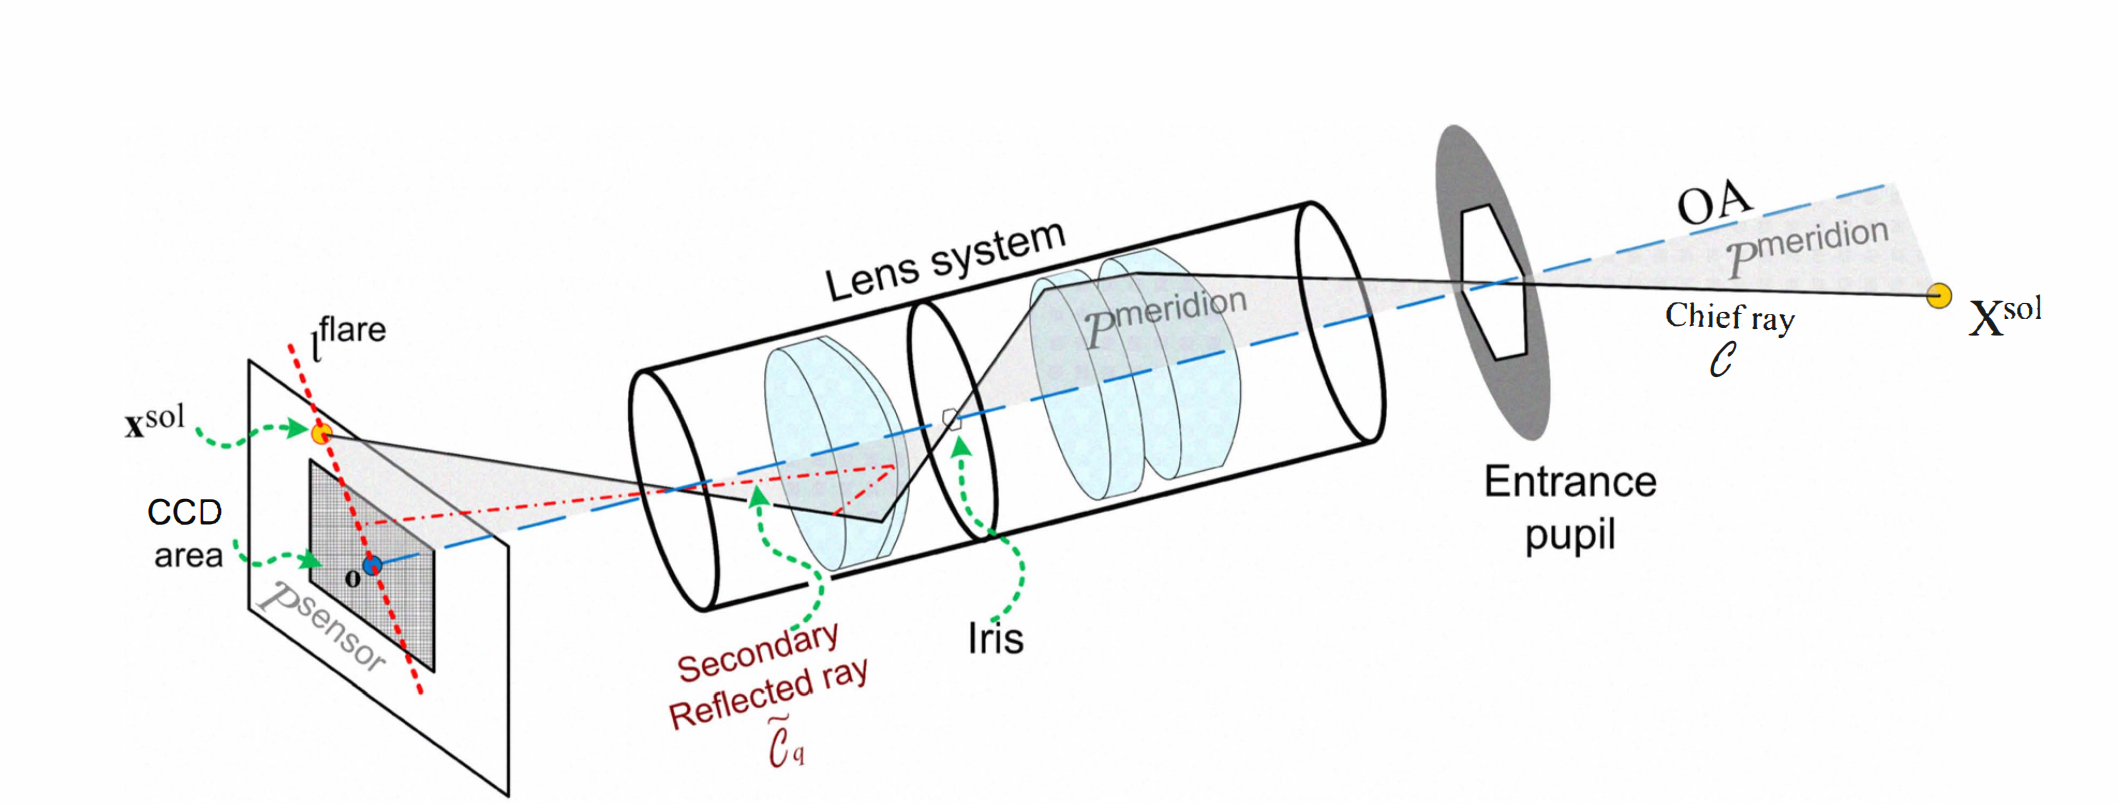
\includegraphics[height=5cm,width=12cm]{20221202.png}
\caption{透镜系统示意图}
\end{figure}
\end{frame}
\begin{frame}
\frametitle{耀斑的去除}
\subsection{图像处理}
取$K_{frames}$个原始图像,记作$G_k(x)$,$k\in[1,K_{frames}]$,各个图像均在相同的场景下拍摄,不同的是在拍摄过程中,相机进行了不规律的移动,进而导致$X_{sol}$在像平面内,对于不同的$k$成了不同的像$x_{sol}$.\pause

由前文所述,对于每个$k$而言,耀斑都应该聚集于一条直线$l^{flare}_k$上,且该直线过光学中心$o$和$x^{sol}_k$\pause

我们假设经过图像的配准(Image Registration),可以使得相机的旋转不仅仅围绕着与平面$P^{meridion}$垂直的轴,进而使得不同$k$对应的直线$l^{flare}_k$互不相同。
\end{frame}
\begin{frame}
\frametitle{去除耀斑}
鉴于在一张图片中,耀斑都聚集在一条直线上,而不同帧数当中的直线互不相同(是运动的)。因此,在某一张图片中被耀斑遮挡的部分,很有可能在其他图片中并未被遮挡。\pause

下面,我们讨论场景或相机运动的补偿(compensate)。图像$k$中的点$\textbf{x}$可以由配准算子$\tau_k$对应到二维全球坐标系(Global 2D coordinate)中的坐标$\textbf{x}_{global}=(x_{global},y_{global})$
对应关系为
\begin{equation}
\textbf{x}_{global}=\tau_k(\textbf{x})
\end{equation}  
如下图所示:
\begin{figure}[!h]
\centering
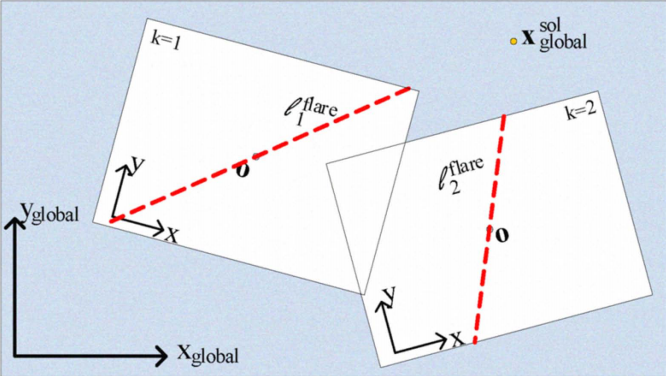
\includegraphics[height=2.5cm,width=5cm]{20221205.png}
\caption{坐标变换示意图}
\end{figure}
\end{frame}    
\begin{frame}
\frametitle{去除耀斑}
经过配准后,方程  
\begin{equation}
G(\textbf{x})=I(\textbf{x})+F(\textbf{x})
\end{equation}                                  
可以转化为
\begin{equation}
\widetilde{G}_k(\textbf{x}_{global})=I(\textbf{x}_{global})+\widetilde{F}_k(\textbf{x}_{global})
\end{equation}   

原始图像和修正后的图像对比如图所示:
\begin{figure}[!h]
\centering
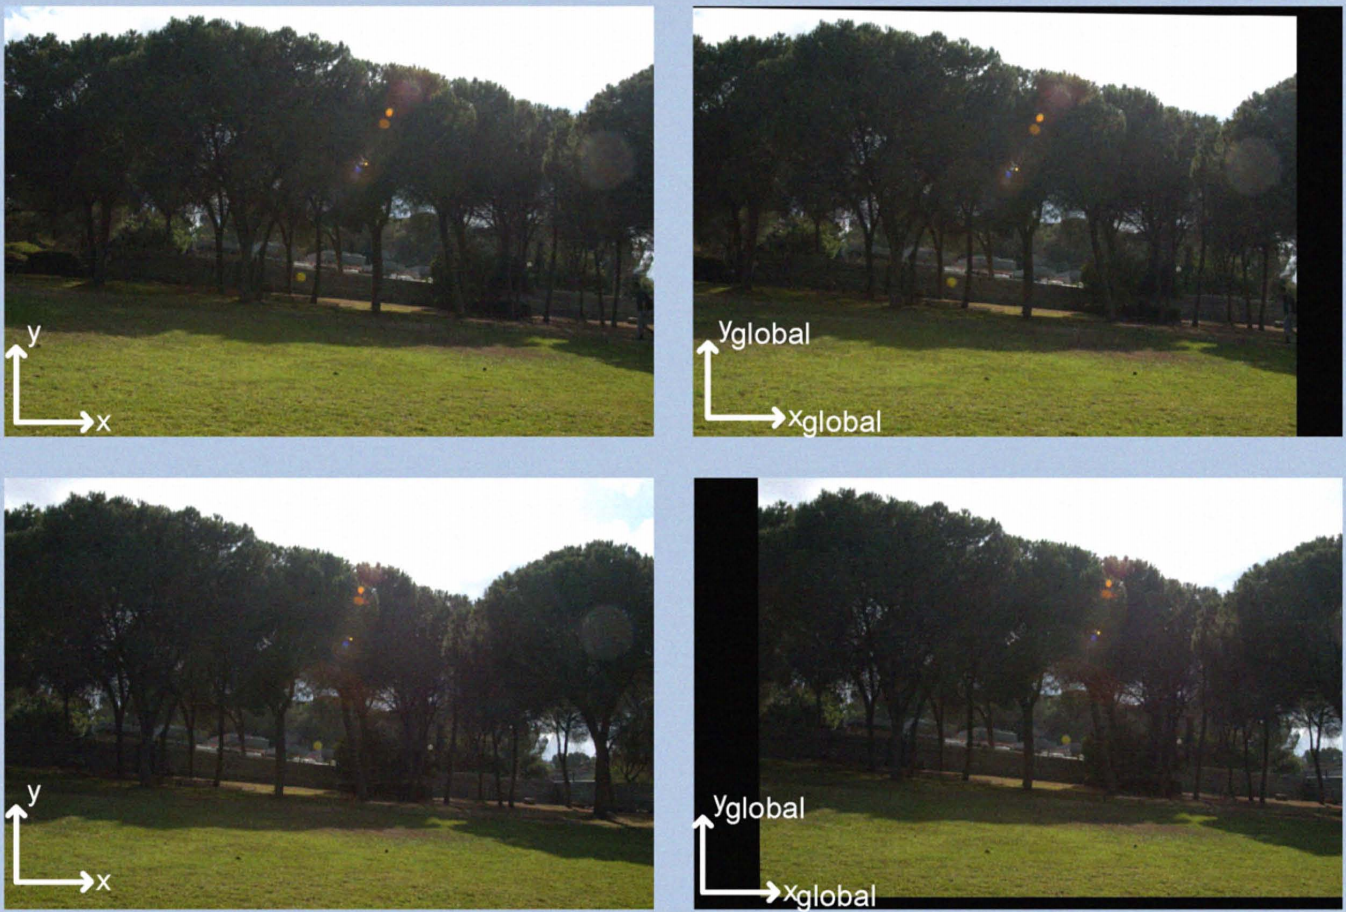
\includegraphics[height=4cm,width=7cm]{2022120501.png}
\caption{对比图}
\end{figure}
\end{frame}
\begin{frame}
\frametitle{去除耀斑}
事实上,在如下公式中
\begin{equation}
\widetilde{G}_k(\textbf{x}_{global})=I(\textbf{x}_{global})+\widetilde{F}_k(\textbf{x}_{global})
\end{equation}   
$I(\textbf{x}_{global})$表示真实世界的景象,其显然与$k$无关,而$\widetilde{F}_k(\textbf{x}_{global})$是随着不同的$k$而变化的\pause

在修正之前,耀斑是随着直线$l_k^{flare}$运动的,且其运动的轨迹与图片的真实运动轨迹并不相同,而修正过程只与$I(\textbf{x}_{global})$有关。因此,修正的过程并不是与耀斑的变化同步的。\pause

对图像中的每个坐标$\textbf{x}_{global}$,总有一组图像在此位置可以\textbf{获取测量值}(acquire measurement),记这组图像为$\Omega(\textbf{x}_{global})$。\pause

由于$\widetilde{F}_k(\textbf{x}_{global})$是恒非负的,因此有下述\textbf{Deflaring Estimator}
\begin{equation}
\hat{I}(\textbf{x}_{global})=\min_{k\in \Omega(\textbf{x}_{global})}\widetilde{G}_k(\textbf{x}_{global})
\end{equation}
\end{frame}
\begin{frame}
\frametitle{确定太阳位置}
由前文所述,耀斑的位置位于太阳的像与图像光学中心的交点处,因此,我们需要估计上述两点的位置。\pause
$X^{sol}$代表太阳位置,其为产生耀斑的光源,记其在图像全球坐标系中的位置为$\textbf{x}_{global}^{sol}$。但是,往往太阳的影像并不会出现在图像当中,因此,我们需要倒推出图像中太阳的位置。本文尝试引入一套打分机制,以此估计太阳在图像中最有可能的位置\pause

由于修正后的$\widetilde{l}_k^{flare}$与修正前的${l}_k^{flare}$等价,因此由前所述,每个$\widetilde{l}_k^{flare}$均穿过太阳的像。因此,如下图所示,直线$\widetilde{l}_k^{flare}$过点$\textbf{x}_{global}^{sol}$.
\begin{figure}[!h]
\centering
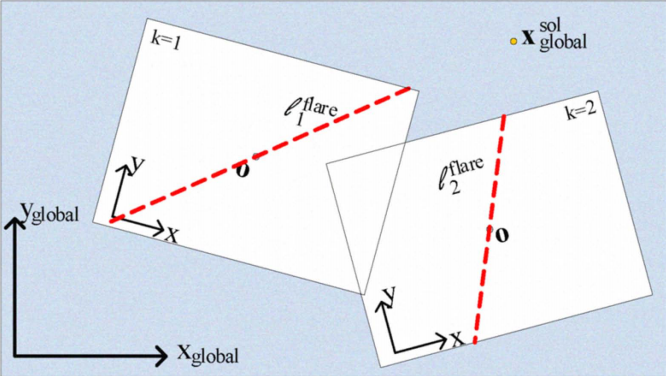
\includegraphics[height=4cm,width=7cm]{20221205.png}
\caption{示意图}
\end{figure}


\end{frame}
\begin{frame}
\frametitle{确定太阳位置}
因此,太阳位置$\textbf{x}_{global}^{sol}$可以视作所有直线$\widetilde{l}_k^{flare}$的交集。\pause

具体而言,在$\textbf{a}$平面中,一条直线可以用向量$\textbf{l}=(r,\theta)$进行描述。其中,$\theta\in[0,\pi]$和$r$的意义见下图:
\begin{figure}[!h]
\centering
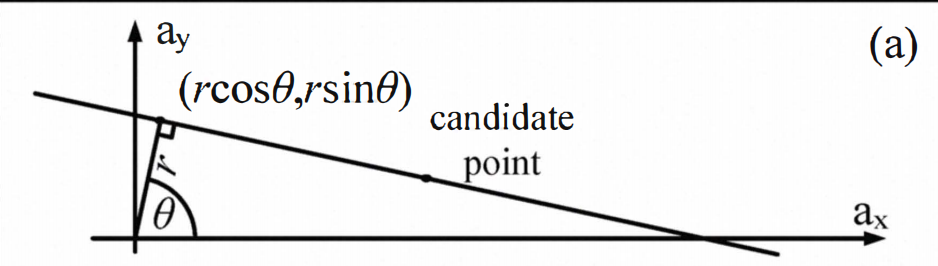
\includegraphics[height=2cm,width=7cm]{2022120502.png}
\caption{$\textbf{l}=(r,\theta)$示意图}
\end{figure}
\end{frame}
\begin{frame}
\frametitle{确定太阳位置}
考虑函数$h(\textbf{a})$的拉东变换(Radon transform)\footnote{若函数 $f(x,y)$ 表示一个未知的密度,对 $f(x,y)$做拉东变换,相当于得到$f(x,y)$ 投影后的信号}

\begin{figure}[!h]
\centering
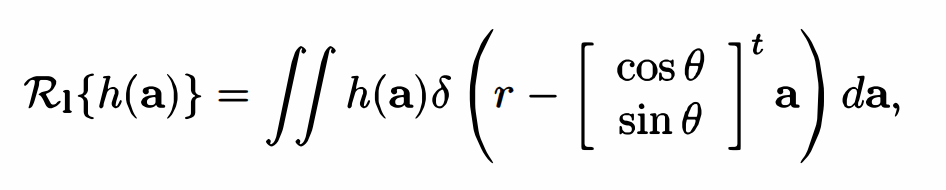
\includegraphics[height=1cm,width=5cm]{2022120503.png}
%\caption{$\textbf{l}=(r,\theta)$示意图}
\end{figure}
其中,$R_1$是拉东变换算子,$t$表示矩阵的转置,$\delta$是狄拉克函数,满足
\begin{equation}
\delta(x)=0,(x\neq0)
\end{equation}
\begin{equation}
\int^{\infty}_{-\infty}\delta(x)dx=1
\end{equation}

\end{frame}
\begin{frame}
\frametitle{确定太阳位置}
取$\textbf{a}=\textbf{x}_{global}$,$h=\hat{\widetilde{F}}_k(\textbf{x}_{global})$,其代表修正后的耀斑图像,满足
\begin{equation}
\hat{\widetilde{F}}_k(\textbf{x}_{global})=\widetilde{G}_k(\textbf{x}_{global})-I(\textbf{x}_{global})
\end{equation}
代入后,得到$R_1\{\hat{\widetilde{F}}_k(\textbf{x}_{global})\}$的值越高,代表直线$l$的得分越高
\end{frame}
\begin{frame}
\frametitle{确定太阳位置}
由下图,我们可知,任何一个可能的太阳像点应该位于这一直线上,
\begin{figure}[!h]
\centering
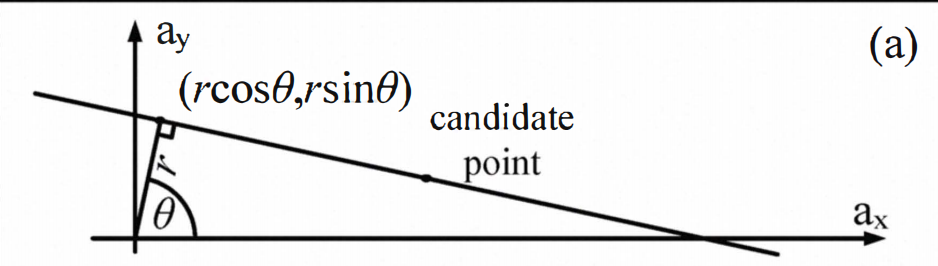
\includegraphics[height=2cm,width=7cm]{2022120502.png}
\caption{$\textbf{l}=(r,\theta)$示意图}
\end{figure}
进而其应该满足如下关系:
\begin{equation}
r=[cos\theta,sin\theta]x_{global}^{candidate}
\end{equation}
\end{frame}
\begin{frame}
\frametitle{确定太阳位置}
因此,不同的$x_{global}^{candidate}$应该对应不同的向量族$\textbf{l}=(r,\theta)$。而这一向量族描述了穿过$x_{global}^{candidate}$点的所有直线,记作$\Lambda x_{global}^{candidate}$如下图所示:
\begin{figure}[!h]
\centering
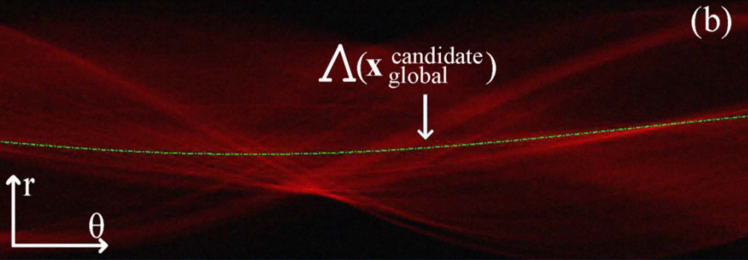
\includegraphics[height=2cm,width=7cm]{2022120504.png}
\caption{$\textbf{l}=(r,\theta)$示意图}
\end{figure}
\end{frame}
\begin{frame}
\frametitle{确定太阳位置}
下面,我们依据上述对直线的打分机制,开始对不同的$x_{global}^{candidate}$进行打分。对于一个图像$k$,$x_{global}^{candidate}$的分数为:
\begin{equation}
s_k(x_{global}^{candidate})=\max_{\textbf{l}\in(x_{global}^{candidate})}R_1\{\hat{\widetilde{F}}_k(\textbf{x}_{global})\}
\end{equation}
得分越高,表明穿过该点$x_{global}^{candidate}$的直线得分越高。
综上,对于一个候选点(candidate point)的总得分为:
\begin{equation}
S(x_{global}^{candidate})=\Sigma_{k=1}^{K_{frames}}s_k(x_{global}^{candidate})\end{equation}
其中得分最高的,即为预估的太阳像点$\hat{\textbf{x}_{global}^{sol}}$
\end{frame}
\begin{frame}
\frametitle{确定太阳位置}
上述过程的示意图见下:
\begin{figure}[!h]
\centering
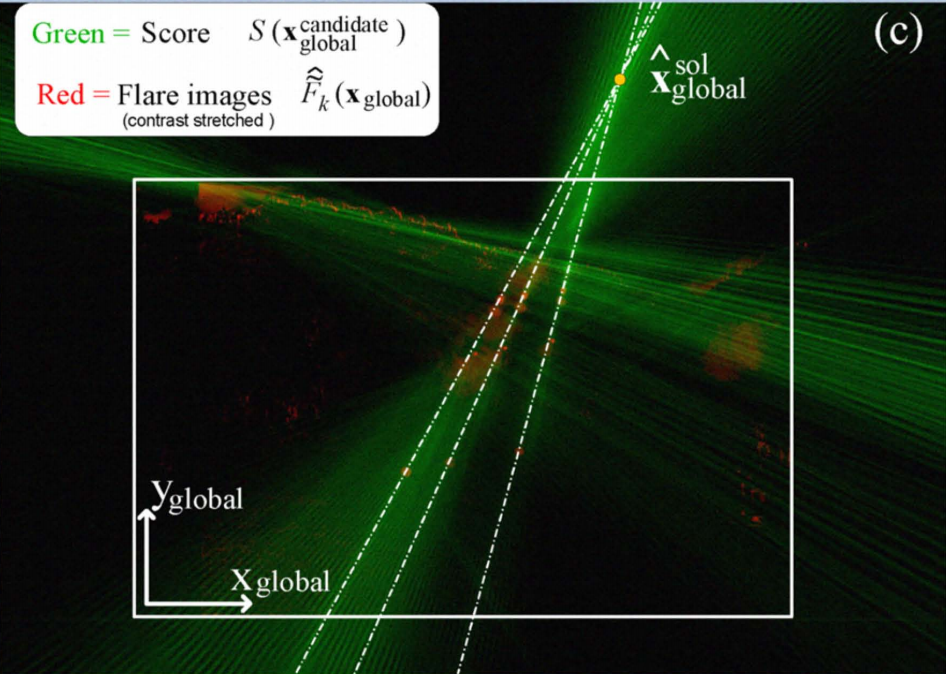
\includegraphics[height=4cm,width=6cm]{2022120505.png}
\caption{示意图}
\end{figure}
\end{frame}
\begin{frame}
\frametitle{光轴位置}
由前所述,每个$l_k^{flare}$均过未修正图像的光学中心$\textbf{o}$,因此,$\textbf{o}$可以看做上述直线的交集。用与太阳定位类似的方法与打分机制,我们可以推测出最有可能的光学中心位置,如下图所示:
\begin{figure}[!h]
\centering
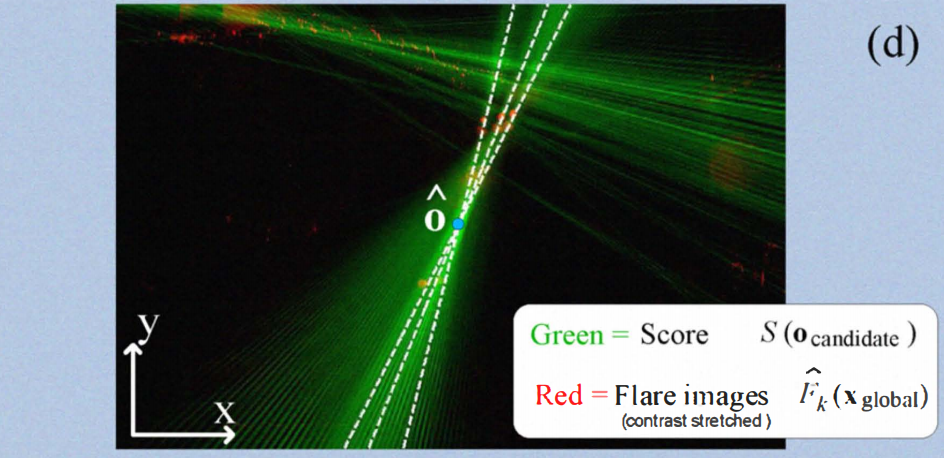
\includegraphics[height=3cm,width=6cm]{2022120506.png}
\caption{示意图}
\end{figure}
\end{frame}
\end{document}